\lecture{2. I will be their God}{02}

\section*{Introduction}

\begin{frame}
\frametitle{God wants a relationship with people}
\framesubtitle{Jeremiah 31:31-34}
	\keyversehiglight{I will be their God}
\end{frame}

\begin{goals}
\goal Consider who God is, and consider how He is similar and different from man.
\goal Explore the different ways God has revealed himself to man.
\goal Think about ways to improve my perspective on who God is.
\end{goals}


\section{Who is God?}

\begin{frame}
\frametitle{God is majestic}
\framesubtitle{Psalm 8}
\begin{center}
	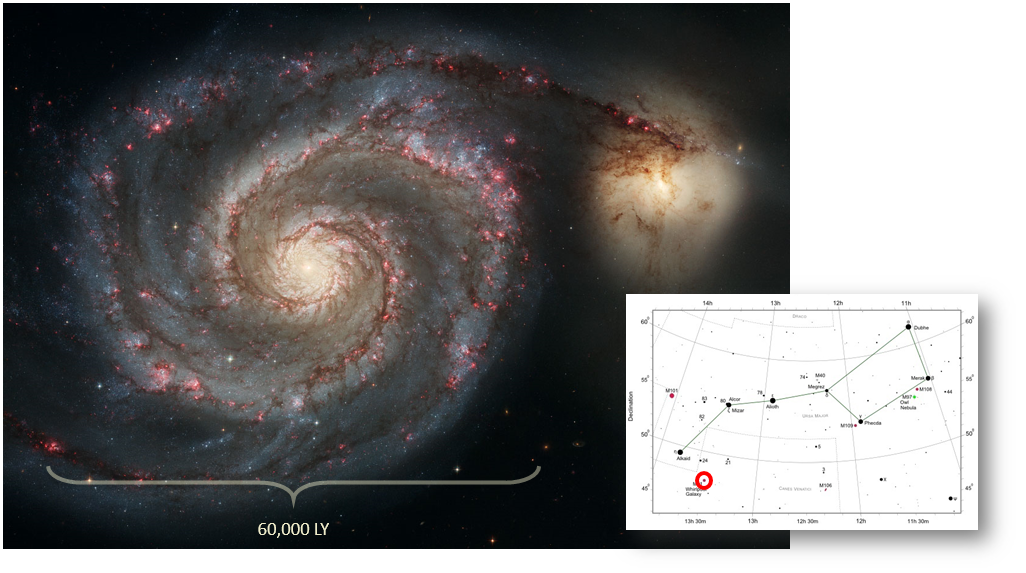
\includegraphics[width=0.85\textwidth]{figures/galaxy.png}\\
	{\footnotesize The Whirlpool galaxy as seen from the Hubble Space Telescope}
\end{center}
\end{frame}

\begin{frame}
\frametitle{God loves man and has blessed him.}
\framesubtitle{Psalm 8}
\begin{center}
	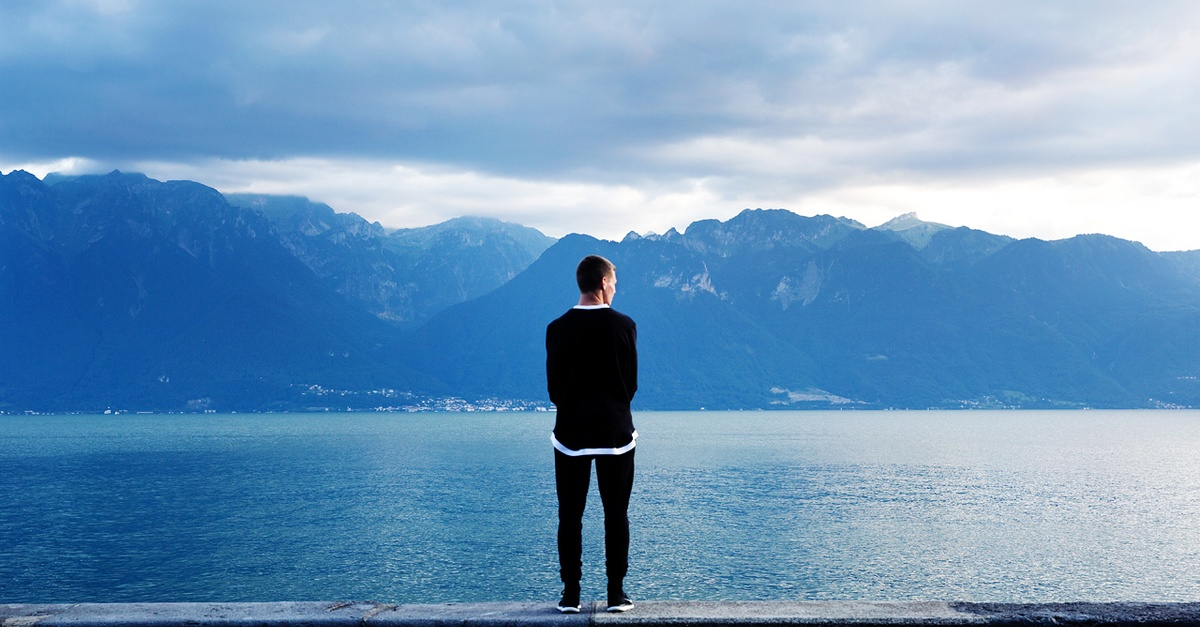
\includegraphics[width=\textwidth]{figures/manLandscape.jpg}
\end{center}
\end{frame}

\section{I will be your God}

\begin{frame}
\frametitle{I will be your God}
\framesubtitle{Gen 17:1-8}
\begin{columns}[T]
	\begin{column}{0.5\textwidth}
	\end{column}
	\begin{column}{0.5\textwidth}
		``And I will give you and to your offspring after you the land of your sojournings, all the land of Canaan, for an everlasting possession, and \alert{I will be  their God}.'' Genesis 17:8\\~\\
	\end{column}
\end{columns}
\end{frame}

\begin{frame}
\frametitle{`I will be their God' through the Bible}
\begin{columns}[T]
	\begin{column}{0.45\textwidth}
		`I will be their God'\\{\footnotesize Gen. 17:8, Jer. 24:7, Jer. 31:33\\Jer. 32:36, Jer. 32:38, Ez. 11:20\\Ez. 37:15, Ez. 37:23, Ez. 37:27\\Zech. 8:8, 2 Cor. 6:16, Heb. 8:10}\\~\\
		`I will be your God'\\{\footnotesize Ex. 6:7, Jer. 7:23, Jer. 11:4\\Jer. 30:2, Ez. 36:28}\\~\\
	\end{column}
	\begin{column}{0.55\textwidth}
			`the Lord your God'\\ 
			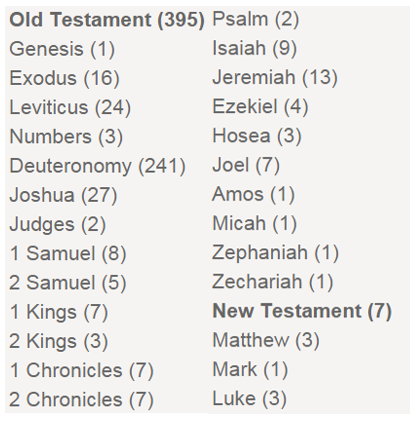
\includegraphics[width=1\columnwidth]{figures/theLordYourGodTwoColumn.png}
	\end{column}
\end{columns}
\note{God also makes a condition with his covenant.  We can infer that God's conditions are necessary because of His might}
\end{frame}

\section{How we come to know about God}

\begin{frame}
\frametitle{Eternity is set in the heart of man}
\framesubtitle{Ecclesiastes 3:11}
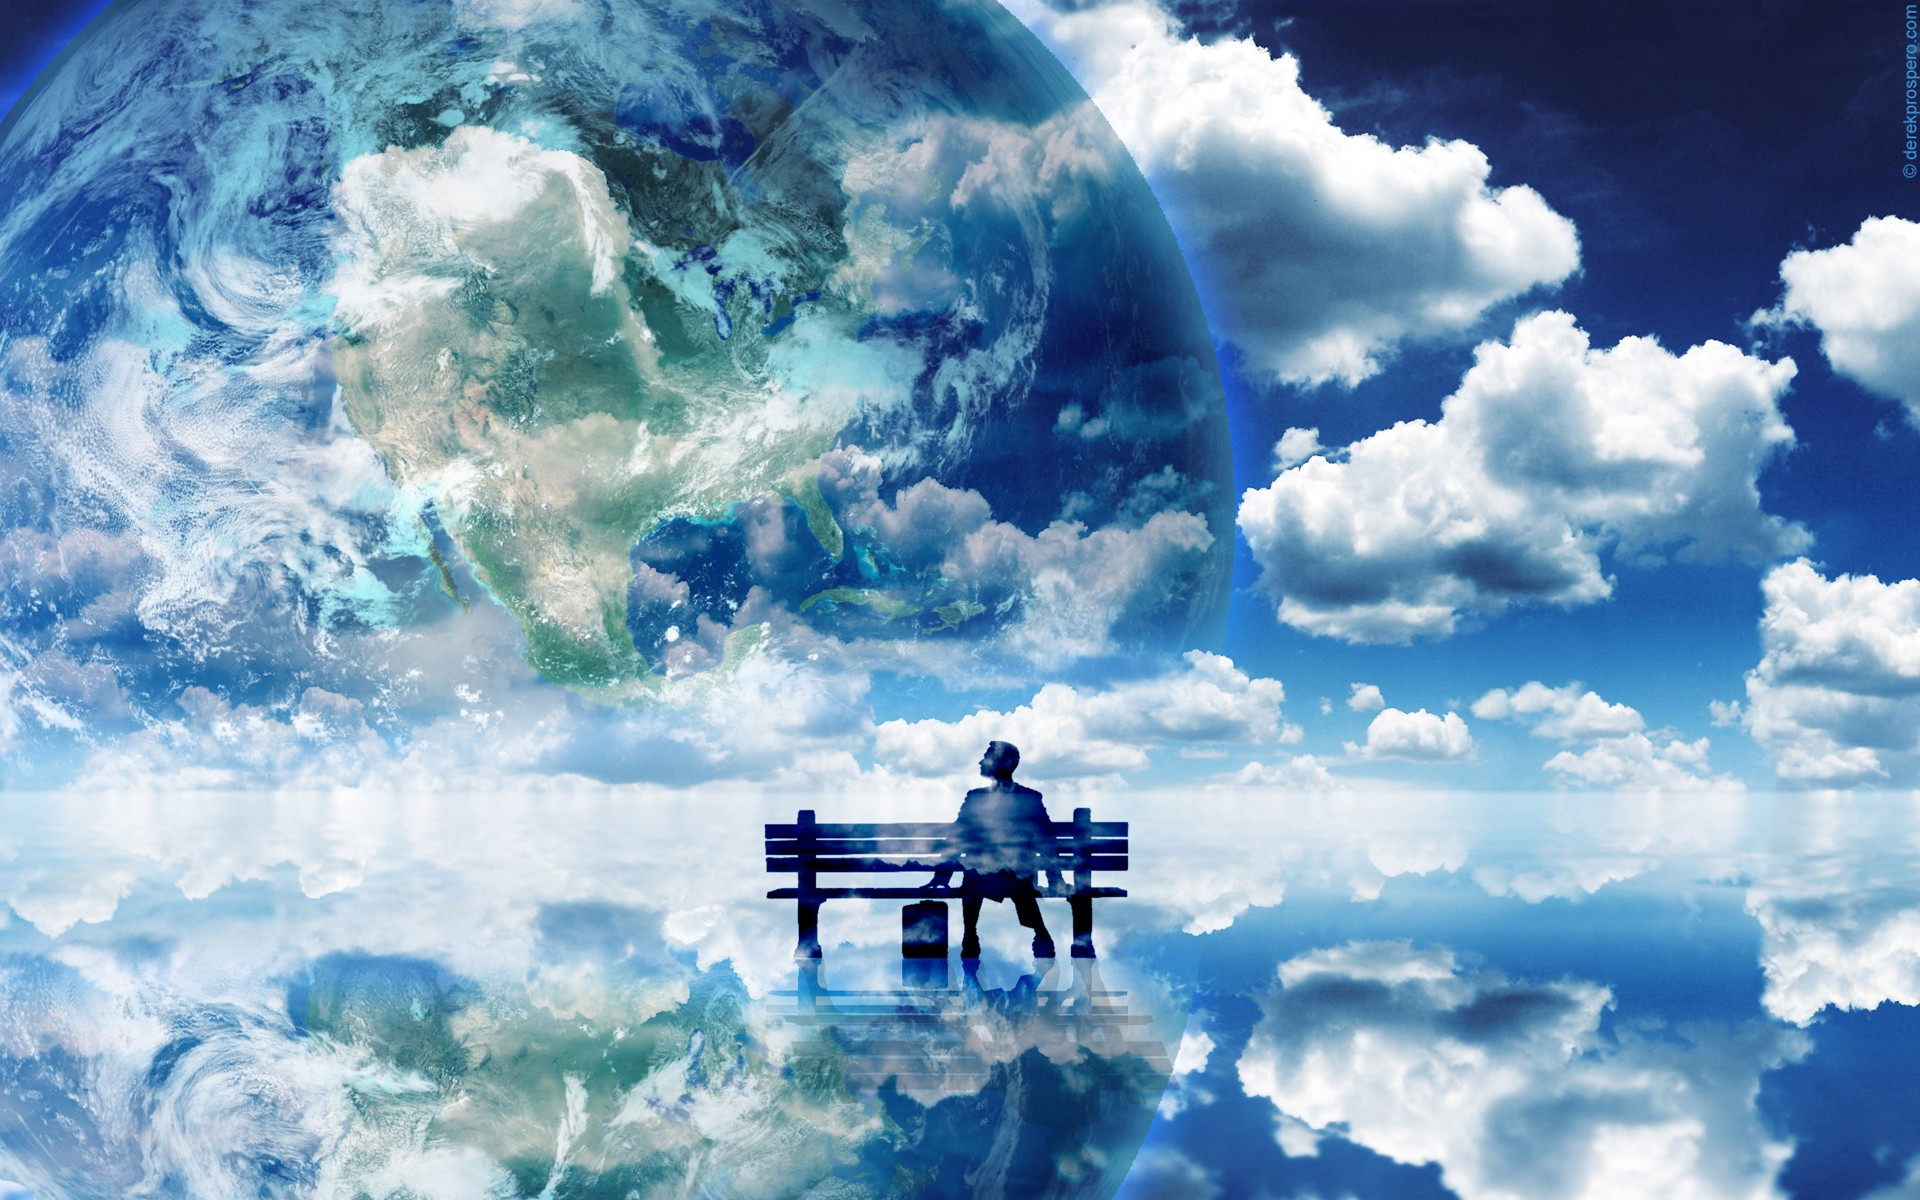
\includegraphics[width=\textwidth]{figures/eternityInHeart.jpg}

\note{God has always made Himself known to man}
\note{However God chose to speak to us, it was going to leverage that part of our being that understands there's something more to life.}
\end{frame}

\begin{frame}
	\frametitle{In the past, he spoke to the Fathers by the prophets}
	\framesubtitle{Hebrews 1:1-2}
\end{frame}

\begin{frame}
	\frametitle{Today, he speaks to us in His Son, Jesus}
	\framesubtitle{Hebrews 1:1-2}
\end{frame}

\begin{frame}
	\frametitle{...And by extension His Word}
	\framesubtitle{Hebrews 1:1-2}
	
\end{frame}

\section{What does that mean for me?}

\begin{frame}
	\frametitle{God gives you moral anchor}
	\framesubtitle{Luke 4:1-13}
	\begin{columns}
	\begin{column}{0.5\textwidth}
	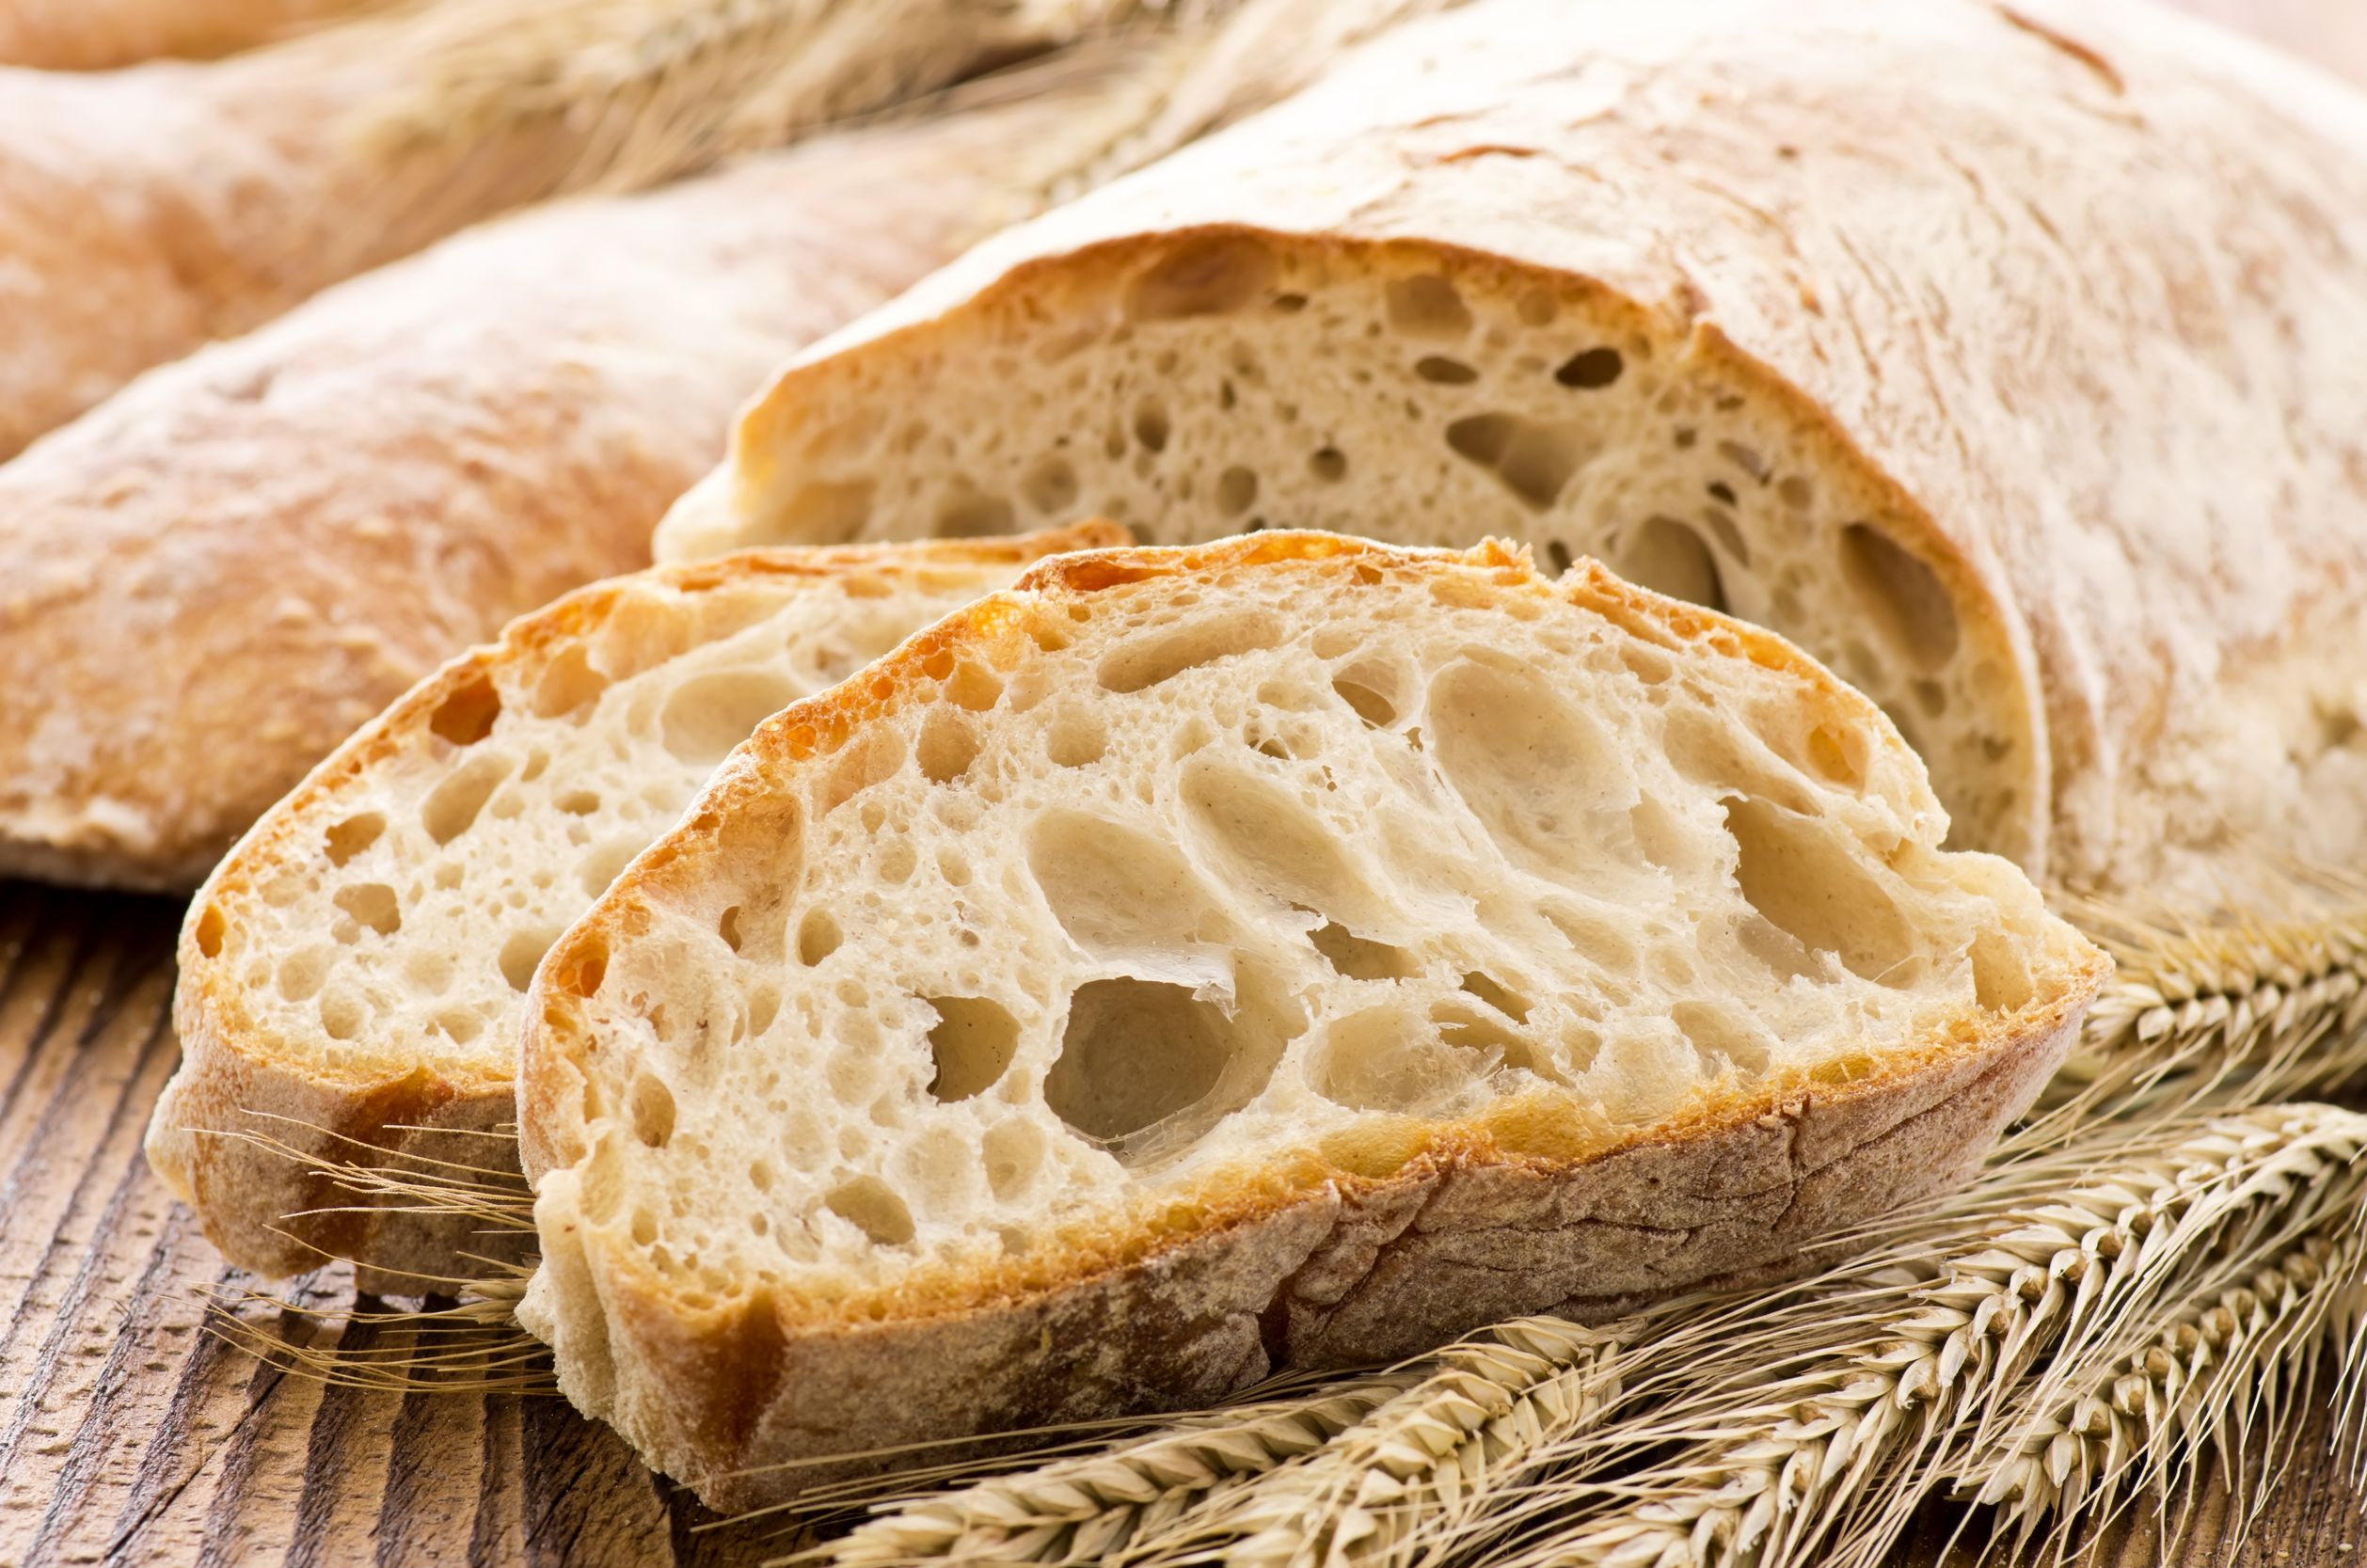
\includegraphics[width=\textwidth]{figures/bread.jpg}
	\end{column}
	\begin{column}{0.5\textwidth}
	\begin{itemize}
	\item Jesus used God as His basis for refuting Satan
	\item There is no objective morality without a God-provided standard
	\note{Atheists don't want an objective morality, until they become disatisfied with their life}
	\end{itemize}
	\end{column}
	\end{columns}
\end{frame}

\begin{frame}
	\frametitle{Loving God is the foundation of eternal life}
	\framesubtitle{Luke 10:25-27}
	\begin{columns}
	\begin{column}{0.5\textwidth}
		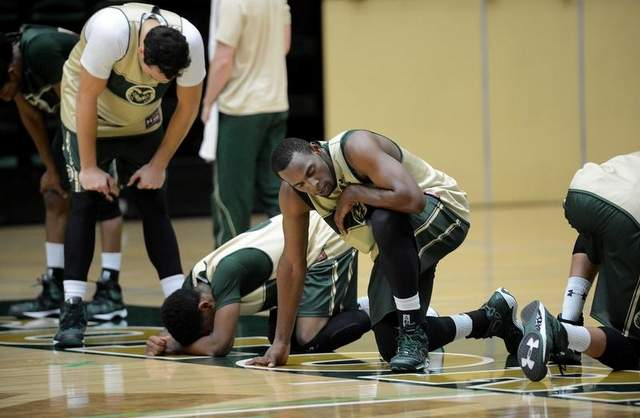
\includegraphics[width=\columnwidth]{figures/basketballRunning.jpg}
	\end{column}
	\begin{column}{0.5\textwidth}
		\begin{itemize}
			\item The main thing is to keep the main thing the main thing. -- {\footnotesize \emph{Steven Covey}}
			\item Sometimes we don't remember what giving all of ourselves looks like.
		\end{itemize}
	\end{column}
	\end{columns}
	\note{We are weak.  And, we are not perfect.  In spite of that, though, we have to keep pushing.  We have to keep trying to give more than we think we can give to God.}
\end{frame}

\section{Review}

\begin{frame}
redo the goals, I think 
\end{frame}